%%%%%%%%%%%%%%%%%%%%%%%%%%%%%%%%%%%%%%%%%
% An unofficial report template for MSc Robotics of the University of Bristol  
% By Tunwu Li (SID 2253543)
%%%%%%%%%%%%%%%%%%%%%%%%%%%%%%%%%%%%%%%%%

\documentclass[12pt]{article}
\usepackage{ctex} % 允许出现中文字符
\usepackage[english]{babel} % Add spaces between languages
\usepackage[utf8x]{inputenc}
\usepackage{amsmath} % Mathematical formulas
\usepackage{xspace}

\usepackage{pdfpages}

\usepackage{graphicx} % For graphics
\usepackage{array} % For formats of tables
\usepackage{multirow} % Merge cells vertically
\usepackage{pythonhighlight} % Python codes
\usepackage{listing} % Codes
\graphicspath{{images/}} % Declare the folder where the images are stored
\usepackage[colorinlistoftodos]{todonotes}
\usepackage{hyperref} % Hyperlinks
\usepackage[hmargin=1.25in,vmargin=1.25in]{geometry} %页边距

\usepackage[noend]{algpseudocode} % for pseudocode
\usepackage{algorithmicx,algorithm}

\usepackage{enumitem} % 编号的缩进
\usepackage{annotate-equations} % Annotated equations

\usepackage[natbibapa]{apacite}
\usepackage{natbib}
\bibliographystyle{apacite} % APA Citation
\setlength{\bibsep}{0pt} % 设置 APA 格式的参考文献段间距为 0

\usepackage{booktabs} % Book-tabs table
\usepackage{subfigure}
% \usepackage{subcaption} % Subheadings for figures and tables

\renewcommand{\thetable}{\thesection{}.\arabic{table}}
\renewcommand{\thefigure}{\thesection{}.\arabic{figure}}
\renewcommand{\theequation}{\thesection{}.\arabic{equation}}
\counterwithin{algorithm}{section}

\linespread{1.0}
\setlength{\parskip}{0.2cm}
\setlength{\parindent}{0pt}


\lstset{language=Matlab,
        alsolanguage=C++,
        tabsize=4,
            frame=shadowbox, % 带阴影的框
            commentstyle=\color{red!10!green!100}, % 绿色注释
            rulesepcolor=\color{red!20!green!20!blue!20}, % 代码块边框为淡青色
            keywordstyle=\color{blue!90}\bfseries, % 关键字为蓝色,粗体
            showstringspaces=false, % 不显示字符串中间的空格标记
            stringstyle=\ttfamily, % 字符串的特殊格式
            keepspaces=true,
            breakindent=22pt,
            numbers=left, % 左侧显示行号
            stepnumber=1, % 行号步长
            numberstyle={\color[RGB]{0,192,192}\tiny}, % 行号字体用小号
            numbersep=8pt,  %设置行号与代码的距离,默认是5pt
            basicstyle=\footnotesize, % 设置代码的大小
            extendedchars=false, % 解决代码跨页时,章节标题、页眉等汉字不显示的问题
            showspaces=false, %
            flexiblecolumns=true, %
            breaklines=true, %对过长的代码自动换行
            breakautoindent=true, %
            breakindent=4em, %
            escapebegin=\begin{CJK*}{GBK}{hei},escapeend=\end{CJK*},
            aboveskip=1em, %代码块边框
            tabsize=2
            % backgroundcolor=\color[rgb]{0.91,0.91,0.91}   %添加背景色
}



%---------------------------------------------------------------------------------

\begin{document}
% \setlength{\parindent}{0pt}
\linespread{1.0} %1.5倍行距

\begin{titlepage}
\linespread{1.0} %标题页1倍行距 
\setlength{\parskip}{0pt} %标题页0段间距
\newcommand{\HRule}{\rule{\linewidth}{0.1mm}} 
\center % Center everything on the page
 
%---------------------------------------------------------------------------------
%	HEADING SECTIONS (Enter the Homework/assignment No., only)
%---------------------------------------------------------------------------------
\textsc{\Large UFMFRR-15-M}\\[0.5cm] % heading course Number
\textsc{\Large Machine Vision}\\[0.5cm] % heading course name
\textsc{\large Group Report}\\[0.5cm] % Minor heading
%---------------------------------------------------------------------------------
%	TITLE SECTION (Replace 'TITLE' with the Homework/assignment Name/title)
%---------------------------------------------------------------------------------

\HRule \\[0.4cm]
{ \huge \bfseries Title}\\[0.1cm] % Title of your Homework/assignment
\HRule \\[1.5cm]
 
%---------------------------------------------------------------------------------
%	AUTHOR SECTION (EDIT THE NAME and T.NO., only)
%---------------------------------------------------------------------------------

\begin{minipage}{0.4\textwidth}
\begin{flushleft} \large

\emph{Authors :}\\ \vspace{0.5em}
First \textsc{Last} \ SID \\ \vspace{0.5em}
First \textsc{Last} \ SID \\ \vspace{0.5em}
\end{flushleft}

\end{minipage}
\begin{minipage}{0.4\textwidth}
\begin{flushright} \large
\emph{Instructor:} \\
Prof \textsc{First Last} \\
Dr \textsc{First Last} % Supervisor's Name
\end{flushright}
\end{minipage}\\[1cm]


\includegraphics[width=0.3\textwidth]{images/University_of_Bristol_logo.png}
\hspace{5mm}

\includegraphics[width=0.25\textwidth]{images/UWE_logo.jpg}
\hspace{5mm}

\includegraphics[width=0.28\textwidth]{images/BRL_logo.PNG}

\vspace{2cm}

{\large \today}\\[1cm] % Date, change the \today to a set date if you want to be precise

\vfill % Fill the rest of the page with white-space

\end{titlepage}
\pagestyle{plain}


%---------------------------------------------------------------------------------
\newpage
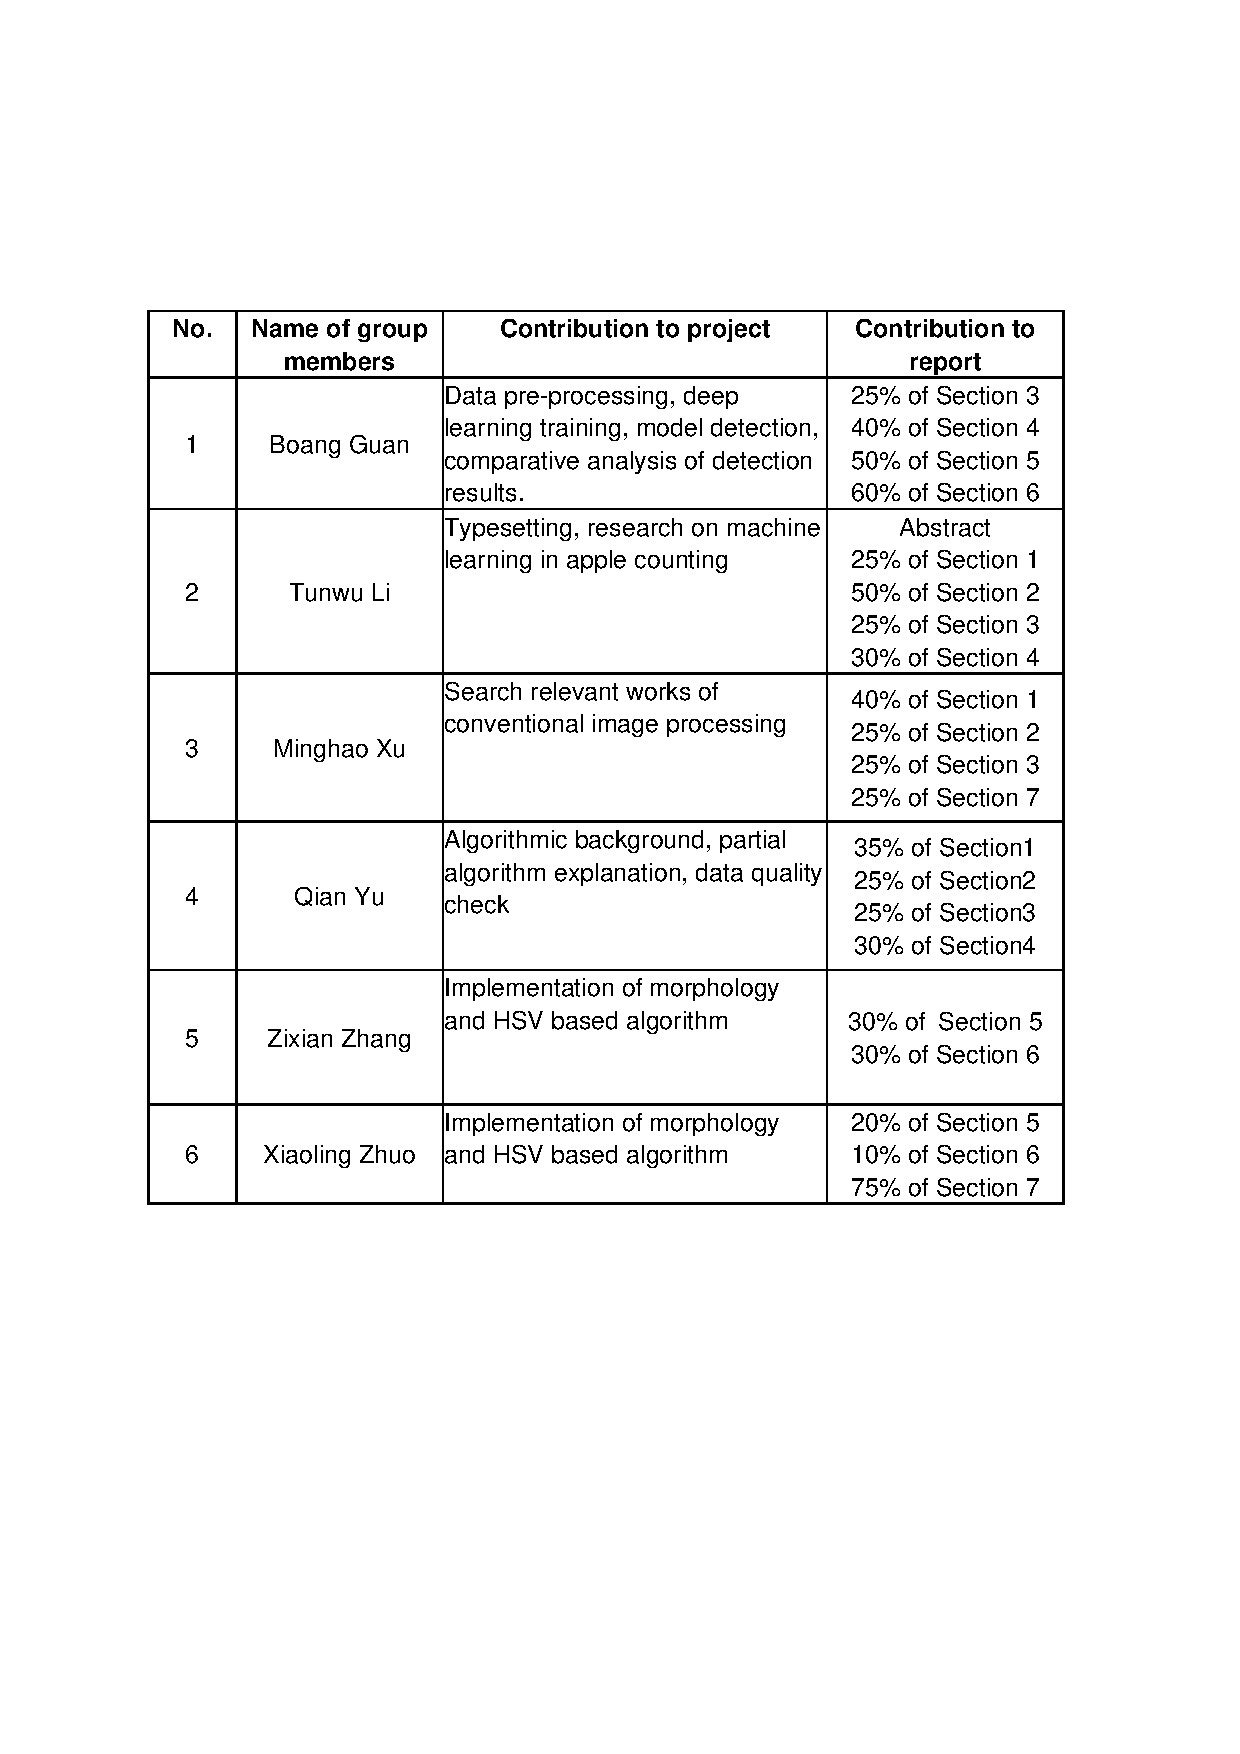
\includepdf{Contribution.pdf} 

\newpage
\linespread{1.0}

\begin{center}
    \section*{Abstract}
\end{center}
\addcontentsline{toc}{section}{Abstract}
\pagenumbering{roman}
This paper is the group work for the Machine Vision course and is divided into ... sections. We present ... in Section~\ref{sec:Intro}.

In Section~\ref{sec:Rel_works}, we summarise ....

Afterwards, in Section~\ref{sec:Data}, we present .... In Section~\ref{sec:Method}, we present ...

We describe in Section~\ref{sec:Experiment} how to ....

We complete the experiments on ... and summarise the results in Section~\ref{sec:Results}.

Conclusions, references and appendices are included at the end, ....




%---------------------------------------------------------------------------------
\newpage
\linespread{1.0}
\setlength{\parskip}{0pt}
\pagestyle{empty}

\tableofcontents % Required
\listoffigures
\listoftables
\thispagestyle{empty}

%---------------------------------------------------------------------------------
\newpage
\linespread{1.0}
\setlength{\parskip}{0.2cm} %段间距0.2cm
\pagestyle{plain}
\setcounter{page}{1}
\pagenumbering{arabic}

% Do not edit the below sections, enter all details in respective chapters
% Add the images/screen-shorts to the image folder and insert them in the respective chapters

\section{Introduction}
\label{sec:Intro}
\subsection{Background}
The rapid growth of ...~\citep{Liu2021}. 

In view of the above background, we try to ....


\subsection{Assumptions}
For the detection task in this paper, we assume that:
\begin{itemize}
    \item ...
    \item ...
    \item ...
\end{itemize}

\subsection{Aims \& Objectives}
We plan to achieve ...:
\begin{itemize}
    \item ...
    \item ...
\end{itemize}

\subsection{Challenges}
After ..., we recognize these challenges:
\begin{itemize}
    \item ...
    \item ...
    \item ...
\end{itemize}



\section{Related Works}
\label{sec:Rel_works}
\subsection{Conventional Image Processing in Apple Counting}
\cite{Qilemuge2018} performed .... 

\cite{Guennouni2014} used .... 


\subsection{Machine Learning in Apple Counting}
\cite{Rahnemoonfar2017} applied .... 

\cite{Chen2017}s' model based on ....


\section{Data Acquisition}
\label{sec:Data}
\subsection{Dataset}
We utilized the MinneApple dataset, collected at the University of Minnesota's Horticultural Research Center (HRC). The dataset contains 1,000 images, which contain approximately 41,000 tagged instances. With a Samsung Galaxy S4 phone, \cite{Haeni2020} took videos of the apple trees moving smoothly on the sunny side, and intercepted every fifth frame of as training datasets and every thirtieth frame as test datasets.

In contrast to COCO, ImageNet, and PASCAL VOC, MinneApple focuses on detecting small objects in cluttered environments, with objects occupying 0.17\% of the image size. The average object categories and numbers of objects in each image for these datasets are summarised in Tab.~\ref{tab:categories}. MinneApple has more instances in a category (41.2), whilst it has fewer categories (1.5). In addition, the MinneApple dataset contains only full resolution images, and the developers took into account the variety of apples and lighting conditions so as to avoid misfitting. 

\begin{table}[htb]
\centering
\caption{Number of categories contained in each image and the number of instances of each category of the four datasets~\citep{Haeni2020}}
\label{tab:categories}
\resizebox{\textwidth}{!}{%
\begin{tabular}{@{}p{4.5cm}<{\centering} p{2.5cm}<{\centering} p{2.5cm}<{\centering} p{2.5cm}<{\centering} p{3cm}<{\centering}@{}}
\toprule
                       & MinneApple & COCO & ImageNet & PASCAL VOC \\ \midrule
Number of categories   & 1.5        & 3.5  & $\le 2$  & $\le 2$    \\
Instances per category & 41.2       & 7.7  & $\le 3$  & $\le 3$    \\ \bottomrule
\end{tabular}%
}
\end{table}


\subsection{Data Quality}
We employ the counting and the detection dataset from the MinneApple, which contains apples of different colours (red, green and yellow), as well as scenes with different light ratios. Most of the images in the counting dataset are $1\ Kb$ in size and have a resolution of no more than $100\times 100$ (Fig.~\ref{fig:counting dataset images}).

\begin{figure}[htb]
    \centering
    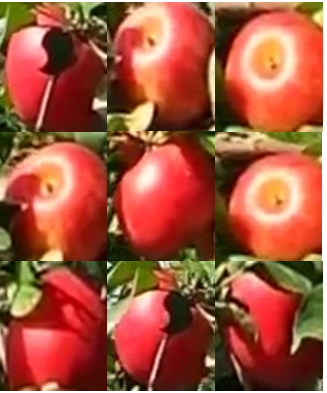
\includegraphics[width=0.3\textwidth]{images/counting_dataset.png}
    \caption{Images from the counting dataset~\citep{Haeni2020}}
    \label{fig:counting dataset images}
\end{figure}

As shown in Fig.~\ref{fig:masked_detection_image}, the annotations in the detection dataset are in the form of Mask. The resolution of the images in the detection dataset is $720\times 1280$, but a small proportion of the photos are overexposed, causing unclear colours and contours and improving the difficulty of the target detection task.

\begin{figure}[htb]
    \centering
    \subfigure[A image from the detection dataset]{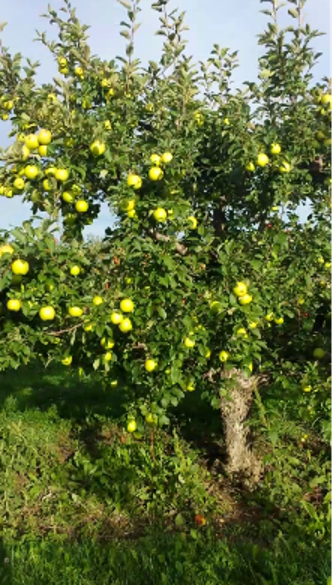
\includegraphics[width=0.3\textwidth]{images/mask_before.png}}
    \subfigure[The annotated image]{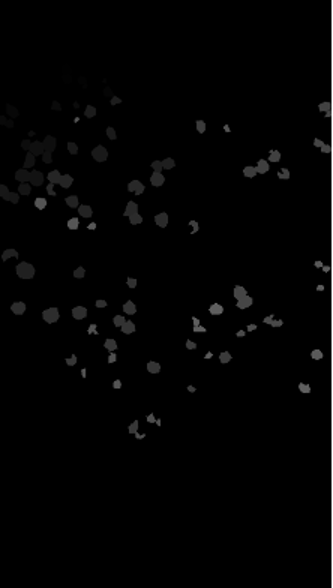
\includegraphics[width=0.3\textwidth]{images/mask_after.png}}
    \caption{A image from the detection dataset and the annotation——(a) a image from the detection dataset and (b) the annotated image}
    \label{fig:masked_detection_image}
\end{figure}





\section{Methodology}
\label{sec:Method}
\subsection{Approach A——Morphology and HSV based Algorithm}
The pseudocode for the morphology and HSV based apple counting method is summarised in Algorithm~\ref{alg:morphological}. Taking the counting test dataset as an example, we first convert the images' colour space to Hue, Saturation, Value (HSV). We then apply inRange thresholding to highlight the foreground. Next, we break two slightly connected foreground regions with morphological opening and draw their contours. Finally, we count all contours with an area greater than $200$ and compare the number with the ground truth, if equal, the task is completed, otherwise it fails. The ratio of all successful cases to the total number of images is the precision. 

\begin{algorithm}[htb]
\label{alg:morphological}
\caption{Morphology and HSV based Algorithm} % 算法的名字
\hspace*{0.02in} {\bf Input:} counting test dataset\\% 算法的输入, \hspace*{0.02in}用来控制位置,\\ 换行
\hspace*{0.02in} {\bf Output:} precision % 算法的结果输出
\begin{algorithmic}[1]

\For{every image in the datasets} % For 语句,需要和EndFor对应
  \State HSV $\gets$ RGB
  \State inRange thresholding (mask)
  \If{$lower\ value \le src(x, y) \le higher\ value$} % If 语句,需要和EndIf对应
    \State $dst(x, y) = 255$
  \Else
    \State $dst(x, y) = 0$
  \EndIf
  \State opening
  \State find contours
  \For{every contour}
      \State calculate the area 
      \If{$area \ge 200$}
          \State $counter \gets counter + 1$
      \Else
          \State continue
      \EndIf
  \State compare counter to ground truth
  \If{$counter == ground\ truth$}
      \State True
  \Else
      \State False
  \EndIf
  \EndFor
\EndFor
\State \Return $precision = \frac{Number\ of\ 'True's}{Number\ of\ images}\times 100\%$
\end{algorithmic}
\end{algorithm}


\subsubsection{HSV}
Hue, Saturation, Value (HSV) is a colour space, commonly used in image processing, in which each colour can be expressed as three digits (Fig.~\ref{fig:HSV diagram}). Compared to RGB, HSV is closer to the perception of colour by human eyes and is therefore beneficial for the extraction of colour features. In the experiment, we identify the target object by setting the HSV range.

\begin{figure}[htb]
    \centering
    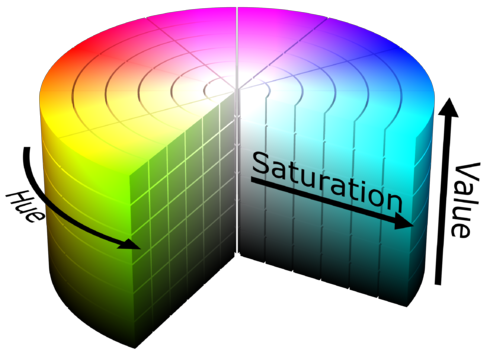
\includegraphics[width=0.35\textwidth]{images/HSV.png}
    \caption{Hue, Saturation, Value colour space (source: \url{https://upload.wikimedia.org/wikipedia})}
    \label{fig:HSV diagram}
\end{figure}

\subsubsection{InRange Thresholding}
InRange thresholding is an image thresholding method with the help of which we create binary images from HSV images, thus separating foreground from background~\citep{Nixon2020}. Specifically, when the source pixel value lies between the two given thresholds, it is assigned a value of 255 and the pixel values outside this range are assigned a value of 0. The expression is as follows:
\begin{equation}
    d(x, y) = \left\{\begin{matrix}
    &255& \quad if\ lower\ value\le s(x, y)\le higher\ value \\
    &0& \quad otherwise
    \end{matrix}\right.
\end{equation}

% \subsubsection{Median Filtering}

% \begin{equation}
%     g(x, y) = med\{f(x-k, y-l)\quad  k, l \in W\}
% \end{equation}

% \begin{figure}[htb]
%     \centering
%     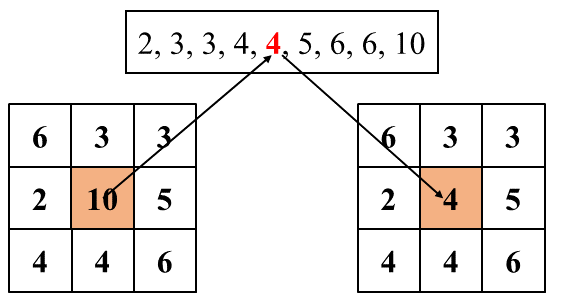
\includegraphics[width=0.4\textwidth]{images/median_filter.png}
%     \caption{Calculation principle of median filtering}
%     \label{fig:princinple of median filtering}
% \end{figure}

\subsubsection{Morphological Opening}
Opening, which is erosion followed by dilation, is used to separate two regions that are finely connected. Erosion and dilation are the two basic operations in morphological processing, on which all other morphological operations are built. The principle of the erosion is to calculate a local minimum in the region of the set kernel and replace the image pixels under the centroid with that value to eliminate the boundary pixel points of the connected regions so that the boundaries shrink inwards, the expression for which is~\citep{OpenCV2022}:
\begin{equation}
    d(x, y) = \eqnmarkbox[blue]{min}{min}_{(x', y')|pixel(x', y')\ne 0}\ s(x+x', y+y')
\end{equation}

where $d(x, y)$ is the destination pixel and the source pixel value ($s(x+x', y+y')$) is replaced by the smallest and non-zero pixel value in the neighbourhood. 

In contrast to erosion, the expansion operation calculates the maximum pixel value that overlaps the kernel and replaces the pixel at the centroid position with that value, resulting in an expansion of the bright region. The expression is~\citep{OpenCV2022}:
\begin{equation}
    d(x, y) = \eqnmarkbox[red]{max}{max}_{(x', y')|pixel(x', y')\ne 0}\ s(x+x', y+y')
\end{equation}

The outcome of the opening operation is shown in Fig.~\ref{fig:'i'}.

\begin{figure}[!ht]
    \centering
    \subfigure[Original 'i']{
\includegraphics[width=0.15\textwidth]{images/origin_i.png}}
    \subfigure[Eroded 'i']{
\includegraphics[width=0.15\textwidth]{images/eroded_i.png}}
    \subfigure[Dilated 'i']{
\includegraphics[width=0.15\textwidth]{images/dilated_i.png}}
    \caption{Eroded and dilated 'i' image~\citep{OpenCV2022}——(a)original 'i', (b) eroded 'i' and (c) dilated 'i'}
    \label{fig:'i'}
\end{figure}


\subsubsection{Contour Finding}
We adopt the Depth-First Search (DFS) algorithm to obtain the contours of the apples (Fig.~\ref{fig:DFS}). The principle is to start traversing down from the starting point and stop when there is no next node~\citep{Gross2003}. This is followed by traversing back to the previous node and continuing in the other direction until all nodes have been traversed.

\begin{figure}[htb]
    \centering
    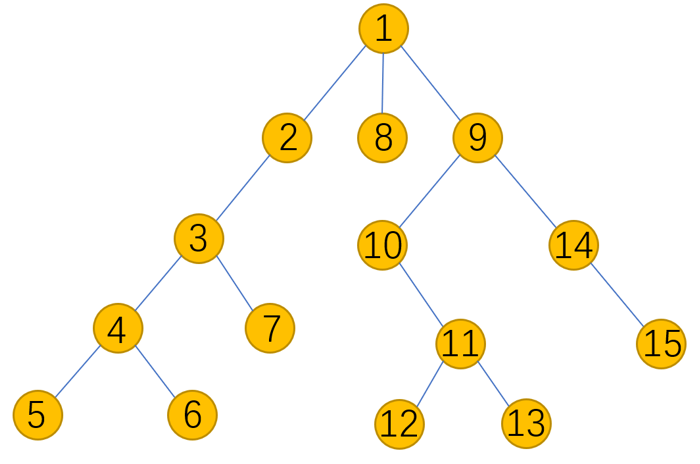
\includegraphics[width=0.4\textwidth]{images/Depth-first-treepng.png}
    \caption{Depth-first search algorithm}
    \label{fig:DFS}
\end{figure}

The advantage of the DFS algorithm is its low time complexity, unless a single route is unusually long. Still, its time complexity is much lower in magnitude than Canny and Sobel. Also, because of the size of the dataset, and the abundance of information in each image, the DFS algorithm is the logical choice.



\subsection{Approach B——Deep Learning}
The network structure of YOLOX (Fig.~\ref{fig:YoloX network structure}) consists of CSPDarknet, Feature Pyramid Network (FPN) and YOLO head. The CSPDarknet is the backbone feature extraction network of YOLOX~\citep{Ge2021}, which composes the extracted features as the input feature set. We acquire three feature layers, namely the effective feature layers, to construct the next network.

\begin{figure}[!ht]
    \centering
    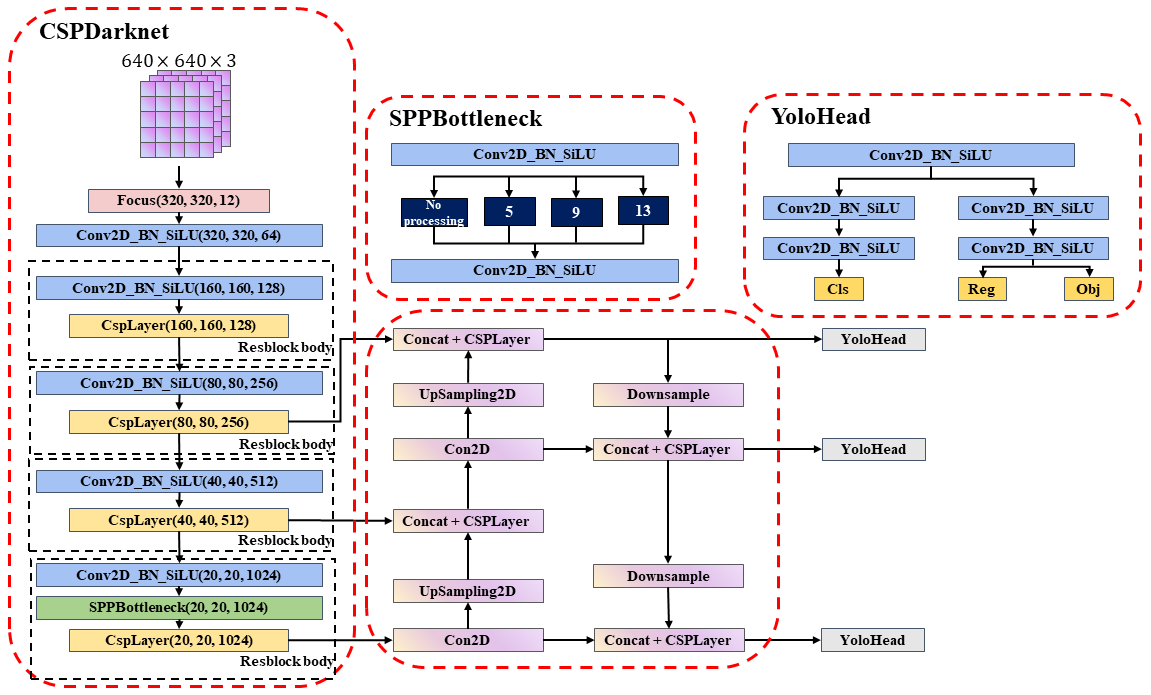
\includegraphics[width=1.1\textwidth]{images/Yolox_structure.png}
    \caption{YOLOX network structure}
    \label{fig:YoloX network structure}
\end{figure}

FPN extracts enhanced features, it fuses the effective feature layers to combine information at various scales. In FPN, we first upsample the features and then downsample them to achieve feature fusion. 

YOLO head is for classification and regression. We treat the previously obtained feature map as an ensemble of feature points, each of which has a number of features per channel. YOLO head determines whether a feature point corresponds to an object or not. Unlike previous versions of YOLO, the YOLO head in YOLOX is divided into two sections, implementing classification and regression respectively, which are integrated when predicting. In summary, the entire YOLOX workflow is: feature extraction, feature enhancement and predicting whether a feature point corresponds to an object or not.


\subsubsection{CSPDarknet}
YOLOX's backbone feature extraction network, CSPDarknet, has four outstanding attributes~\citep{Ge2021}.
\begin{enumerate}
    \item \textbf{The residual network.} The backbone of the residual convolution is the combination of a $1\times 1$ convolution and a $3\times 3$ convolution, with the residual edge portion incorporating the input and output of the backbone. By increasing the depth, the residual network can be optimised, thus improving the model's accuracy since the internal residual blocks are connected in a leap form to mitigate gradient disappearance. 
    
    \item \textbf{CSPNet.} The stacked residual blocks are dissected into two halves as shown in Fig.~\ref{fig:CSPnet}, with the backbone handling to continue to stack the residual blocks and the other part is similar to the residual edge and is joined to the end with little processing.
    
        \begin{figure}[htb]
            \centering
            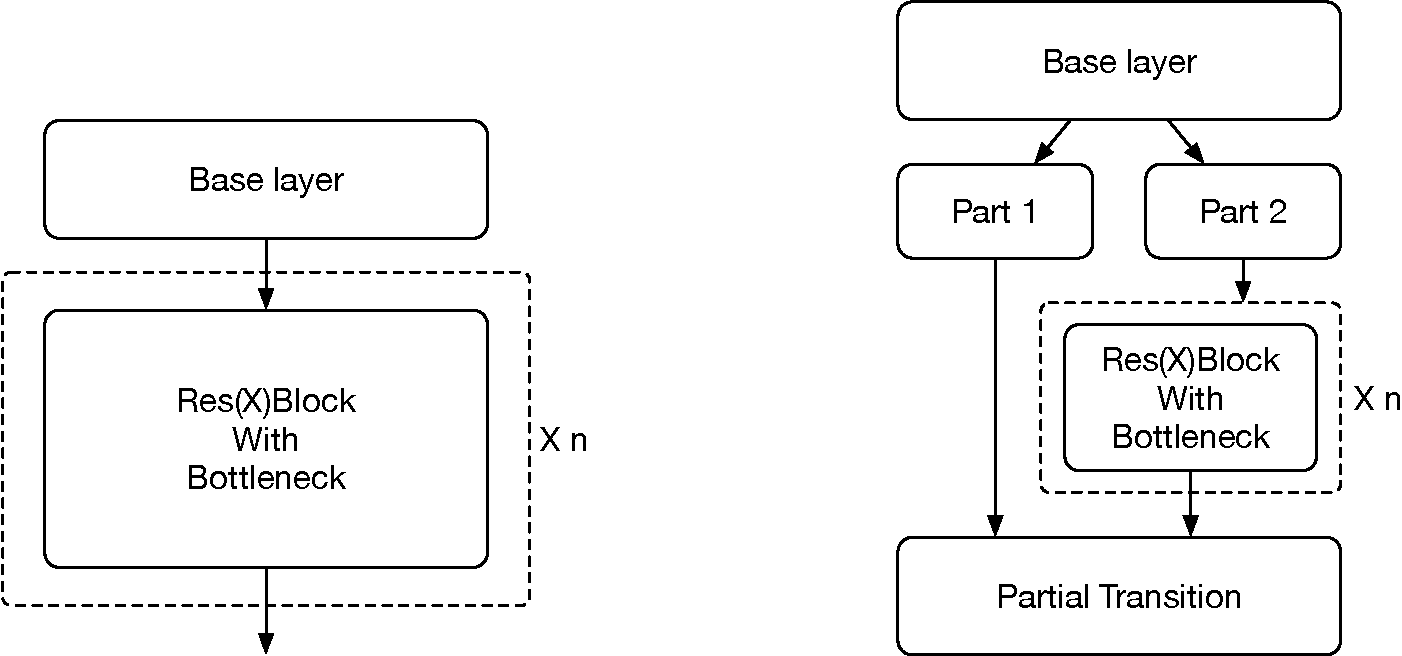
\includegraphics[width=0.6\textwidth]{images/Fig 4.7.pdf}
            \caption{CSPNet in the CSPDarknet}
            \label{fig:CSPnet}
        \end{figure}
    
    \item \textbf{Focus network structure.} As shown in Fig.~\ref{fig:Focus}, a value is taken every other pixel in an image to obtain four separate feature layers. Then stack the four separate feature layers thereby brings the width and height information into the channel information and the input channels are enlarged by four times (three channels → twelve channels).
    
        \begin{figure}[htb]
            \centering
            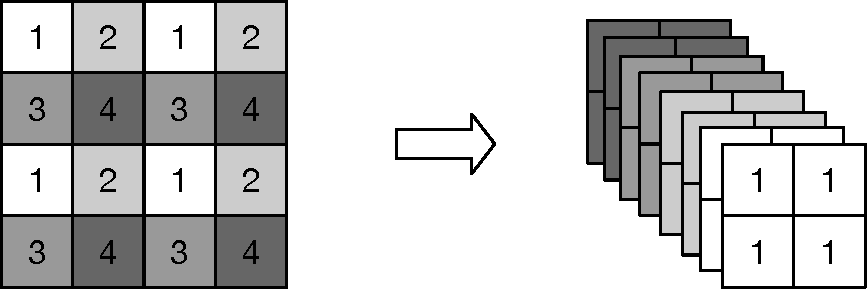
\includegraphics[width=0.5\textwidth]{images/Fig 4.8.pdf}
            \caption{Focus network structure}
            \label{fig:Focus}
        \end{figure}
    
    \item \textbf{SiLU activation function.} As shown in Fig.~\ref{fig:SiLU}, SiLU has the properties of being unbounded with a lower bound, smooth and non-monotonic~\citep{Elfwing2018}, and can be described as a smooth version of ReLU, which outperforms ReLU in deep models.
    
        \begin{figure}[htb]
            \centering
            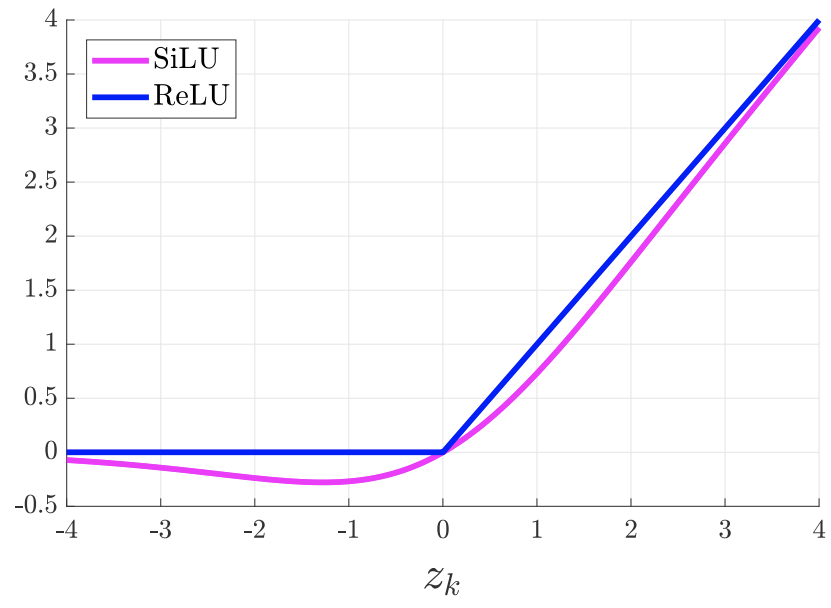
\includegraphics[width=0.5\textwidth]{images/SiLU.png}
            \caption{Curves of SiLU and ReLU activation functions~\citep{Elfwing2018}}
            \label{fig:SiLU}
        \end{figure}
    
\end{enumerate}


\subsubsection{Feature Pyramid Network}
In the feature utilisation phase, the three feature layers are situated in the middle, lower middle and bottom layers of the CSPDarknet (Fig.~\ref{fig:YoloX network structure}). When the input is $640\times 640\times 3$, the shapes of the three feature layers are: $feat_1 = 80\times 80\times 256$, $feat_2 = 40\times 40\times 512$ and $feat_3 = 20\times 20\times 1024$. The feature pyramid merges features with feature layers of different shapes to facilitate the extraction of more detailed features, and we build the FPN through the three effective feature layers.


\subsubsection{Decoupled YOLO Head}
We gain three enhanced features with dimensions of $80\times 80\times 256$, $40\times 40\times 512$ and $20\times 20\times 1024$ by FPN and pass them into YOLO head for prediction~\citep{Elfwing2018}. For each feature layer, we obtain three predictions, as shown in Fig.~\ref{fig:YOLO head}:
\begin{itemize}
    \item $Regression\ (h\times w\times 4)$——determines the regression parameters of the feature points, used to obtain the prediction bounding box.
    \item $Object\ (h\times w\times 1)$——determines if the feature point includes an object.
    \item $Classification\ (h\times w\times num\_classes)$——determines the class of the object contained in each feature point.
\end{itemize}

\begin{figure}[htb]
    \centering
    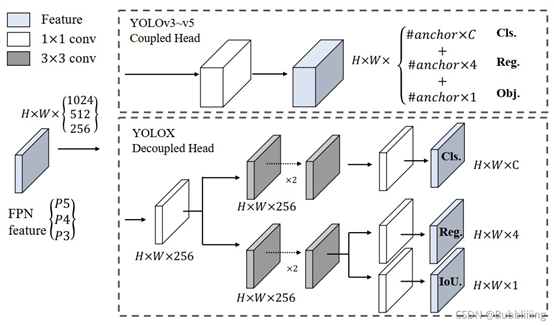
\includegraphics[width=0.65\textwidth]{images/YoloHead.png}
    \caption{Network structure of the YOLO heads within different versions of YOLO (source: \url{https://blog.csdn.net})}
    \label{fig:YOLO head}
\end{figure}

Stack the three predictions above, then the output of each feature layer is $h\times w\times (4 + 1 + num\_classes)$.


\subsubsection{Scoring Screening with Non-maximal Suppression}
We first find the prediction boxes with scores greater than the threshold function in the prediction outcomes. Subsequently, we apply non-maximal suppression to each class and sort them by score from highest to lowest. At last, we calculate the overlap of the highest scoring box with all other boxes and eliminate those with excessive overlap. The predictions without non-maximum suppression and with non-maximum suppression are shown in Fig.~\ref{fig:non-max suppression}.

\begin{figure}[htb]
    \centering
    \subfigure[Predictions before non-maximal suppression]{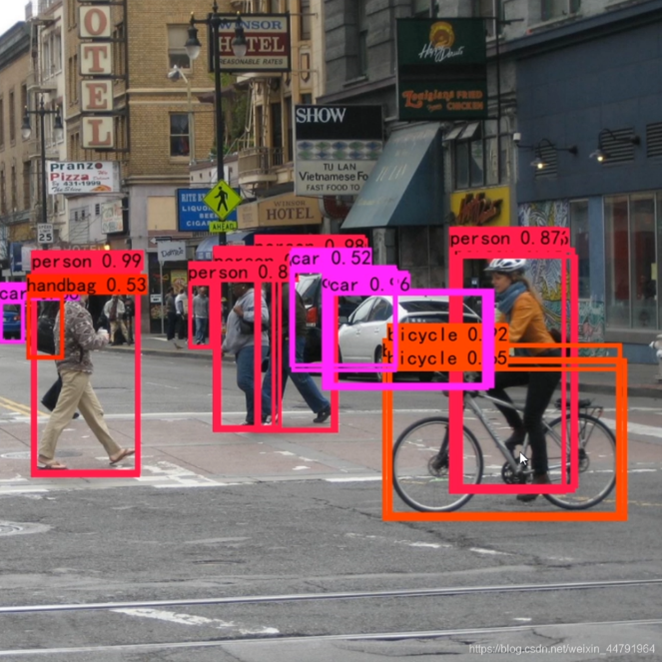
\includegraphics[width=0.4\textwidth]{images/non-max suppression_left.png}}
    \subfigure[Predictions after non-maximal suppression]{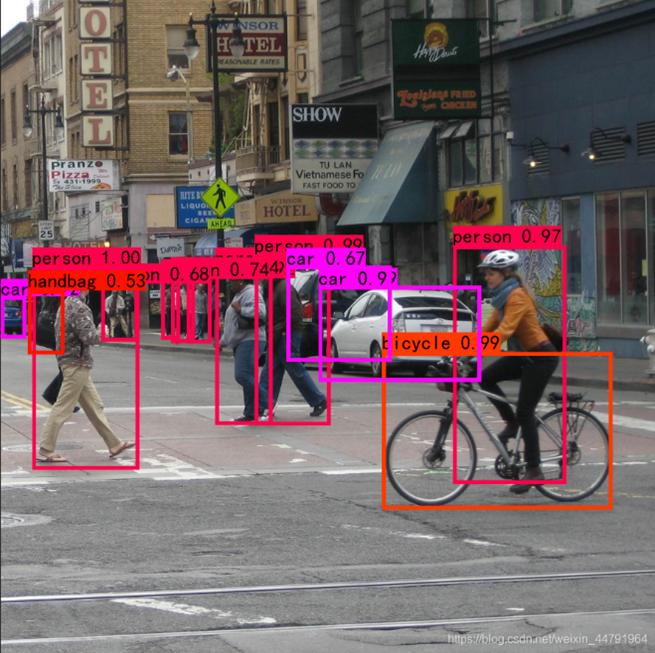
\includegraphics[width=0.4\textwidth]{images/non-max suppression_right.png}}
    \caption{Predictions before and after non-maximal suppression——(a) before and (b) after (source: \url{https://towardsdatascience.com})}
    \label{fig:non-max suppression}
\end{figure}


\section{Experiment and Implementation}
\label{sec:Experiment}
We executed our experiments on ...


\subsection{Experiment A——}

\subsubsection{Determination of ...}
...

\subsubsection{Determination of ...}
...


\subsection{Experiment B——}

\subsubsection{Dataset preparation}
... 

\subsubsection{Pre-processing of the Dataset}
...


\subsubsection{Training}
The hardware ... and the training hyperparameters are listed in Tab.~\ref{tab:Hyperparameters} and Tab.~\ref{tab:Hardwares}.

\begin{table}[htb]
\centering
\caption{Hardwares and their parameters}
\label{tab:Hardwares}
\resizebox{\textwidth}{!}{%
\begin{tabular}{@{}p{7cm}<{\centering} p{7cm}<{\centering}@{}}
\toprule
Hardware & Parameter                       \\ \midrule
GPU      &           \\
VRAM     &                        \\
CPU      &  \\
RAM      &                         \\ \bottomrule
\end{tabular}%
}
\end{table}

\begin{table}[htb]
\centering
\caption{Hyperparameters for training}
\label{tab:Hyperparameters}
\resizebox{\textwidth}{!}{%
\begin{tabular}{@{}p{7cm}<{\centering} p{7cm}<{\centering}@{}}
\toprule
Hyperparameter        & Value        \\ \midrule
Input shape           &  \\
Epoch                 &          \\
Batch size            &           \\
Initial learning rate  &          \\
Minimum learning rate &       \\
Optimizer             &         \\
Activation function   &  \\ \bottomrule
\end{tabular}%
}
\end{table}

The curve of the loss and the mean Average Precision (mAP) along epochs is shown in Fig. .




\section{Results and Evaluation}
\label{sec:Results}
\subsection{Metrics}
...

\subsection{Results A——}
The results of ... are summarised in Tab.~\ref{tab:results_1}. We achieved ...

\begin{table}[htb]
\centering
\caption{Results of ...}
\label{tab:results_1}
\resizebox{\textwidth}{!}{%
\begin{tabular}{@{}p{5cm}<{\centering} p{5cm}<{\centering} p{5cm}<{\centering}@{}}
\toprule
Dataset   & Precision & Running time/s \\ \midrule
Counting  &  &        \\
Detection &  &       \\ \bottomrule
\end{tabular}%
}
\end{table}

\subsubsection{Result in the counting dataset}
... 


\subsubsection{Result in the detection dataset}
...


\subsection{Results B——}
The results of ... are summarised in Tab.~\ref{tab:results_2}. It achieved ...

\begin{table}[htb]
\centering
\caption{Results of ...}
\label{tab:results_2}
\resizebox{\textwidth}{!}{%
\begin{tabular}{@{}p{5cm}<{\centering} p{5cm}<{\centering} p{5cm}<{\centering}@{}}
\toprule
Dataset   & Precision & Running time/s \\ \midrule
Counting  &  &       \\
Detection &  &       \\ \bottomrule
\end{tabular}%
}
\end{table}

\subsubsection{Result in the counting dataset}
...


\subsubsection{Result in the detection dataset}
...


\subsection{Comparison}

\subsubsection{Running Time}
To be fair, we turned off the GPU acceleration and ... The results are listed in Tab.~\ref{tab:running_time_test}.

We found that ... 

\begin{table}[htb]
\centering
\caption{Results of the running time tests}
\label{tab:running_time_test}
\resizebox{\textwidth}{!}{%
\begin{tabular}{@{}p{7cm}<{\centering} p{4cm}<{\centering} p{4cm}<{\centering}@{}}
\toprule
                                   & Counting dataset & Detection dataset \\ \midrule
Algorithm 1 &         &          \\
... without GPU                              &          &             \\ \bottomrule
\end{tabular}%
}
\end{table}


\subsubsection{Precision}
... 

\subsubsection{Energy-precision Ratio}
... The expression is:

\begin{equation}
    \left\{\begin{matrix}
    R = \frac{A}{W}  \\
    W = \sum p_h\times T
    \end{matrix}\right.
\end{equation}

where $W$ is ..., which gives the... in Tab.~\ref{tab:energy-accuracy ratio test}.

\begin{table}[htb]
\centering
\caption{The results of the energy-precision ratio test}
\label{tab:energy-accuracy ratio test}
\resizebox{\textwidth}{!}{%
\begin{tabular}{@{}p{7cm}<{\centering} p{4cm}<{\centering} p{4cm}<{\centering}@{}}
\toprule
                                   & Counting dataset       & Detection dataset      \\ \midrule
Algorithm 1 &                &                \\
... with GPU                     &  &  \\
... without GPU                  &  &  \\ \bottomrule
\end{tabular}%
}
\end{table}

\subsubsection{Overall Analysis}
...

\section{Conclusions and Future Works}
\label{sec:Conclusions}
In conclusion, ...

Nonetheless, ...

One of the future works is ... 

Moreover, we believe that ...

% \nocite{*}
\bibliography{References}
\addcontentsline{toc}{section}{References}

\newpage
\pagestyle{empty}
\section*{Appendix A Python Codes of Morphology and HSV based Algorithm on Counting Test Dataset}
\addcontentsline{toc}{section}{Appendix A Python Codes of Morphology and HSV based Algorithm on Counting Test Dataset}
\begin{python}
import csv
import cv2
import numpy as np
import os
import pandas as pd
import time

# 读取图像并转换为 HSV 颜色空间
def counting(image):

    hsv = cv2.cvtColor(image, cv2.COLOR_BGR2HSV)

    # 设定红色和绿色的颜色范围
    lower_red1 = np.array([0,43,15])
    upper_red1 = np.array([34,255,255])
    lower_red2 = np.array([156,43,15])
    upper_red2 = np.array([180,255,255])
    lower_green = np.array([78,43,15])
    upper_green = np.array([90,255,255])

    # 限制图像在红色和绿色范围内
    mask1 = cv2.inRange(hsv, lower_red1, upper_red1)
    mask2 = cv2.inRange(hsv, lower_red2, upper_red2)
    mask3 = cv2.inRange(hsv, lower_green, upper_green)

    # 合并两个 mask
    mask = mask1 + mask2 + mask3

    # 去除噪声
    kernel = cv2.getStructuringElement(cv2.MORPH_ELLIPSE, (3,3))
    mask = cv2.morphologyEx(mask, cv2.MORPH_OPEN, kernel, iterations = 5)

    # 找到苹果的轮廓
    contours, _ = cv2.findContours(mask, cv2.RETR_TREE, cv2.CHAIN_APPROX_SIMPLE)

    # 绘制轮廓
    countapple = 0

    for contour in contours:
        area = cv2.contourArea(contour)
        k = cv2.isContourConvex(contour)
        if area >200:
            countapple = countapple + 1
        x,y,w,h = cv2.boundingRect(contour)
        image = cv2.rectangle(image, (x,y), (x+w,y+h), (0,255,0), 2)
    return countapple

# 显示结果图像
# cv2.imshow('Image', image)
# cv2.waitKey(0)
# print(countapple)
mainFolder = "val/images"

def getPhoto():
    path_photo = 'images'
    files_list = os.listdir(path_photo)
    #
    print(type(files_list))
    print(files_list)
array_of_img = []
def read_directory(directory_name):

    for filename in os.listdir(r"./"+directory_name):
        img = cv2.imread(directory_name + "/" + filename)
        array_of_img.append(img)

read_directory("images")


data = pd.read_csv("ground_truth.csv")
with open("ground_truth.csv", 'r') as f:
    reader = csv.reader(f)
    result = list(reader)
y = result[1]
y = list(map(int,y))
# print(y)

returntrue = 0
start_time = time.time()
for i in range(0,len(array_of_img)):
    # print(counting(array_of_img[i]))
    if counting(array_of_img[i]) ==y[i]:
        returntrue = returntrue +1

rate = returntrue/len(array_of_img)
end_time = time.time()
print('get \%f acc' \% (rate-0))
print('cost \%f second' \% (end_time - start_time))
\end{python}
\thispagestyle{empty}

\newpage
\pagestyle{empty}
\section*{Appendix B Python Codes of Morphology and HSV based Algorithm on Detection Test Dataset}
\addcontentsline{toc}{section}{Appendix B Python Codes of Morphology and HSV based Algorithm on Detection Test Dataset}
\begin{python}
import csv
import cv2
import numpy as np
import os
import pandas as pd
import time


# 读取图像并转换为 HSV 颜色空间
def counting(image):
    hsv = cv2.cvtColor(image, cv2.COLOR_BGR2HSV)

    # 设定红色和绿色的颜色范围
    lower_red1 = np.array([0, 43, 15])
    upper_red1 = np.array([34, 255, 255])
    lower_red2 = np.array([156, 43, 15])
    upper_red2 = np.array([180, 255, 255])
    lower_green = np.array([78, 43, 15])
    upper_green = np.array([90, 255, 255])

    # 限制图像在红色和绿色范围内
    mask1 = cv2.inRange(hsv, lower_red1, upper_red1)
    mask2 = cv2.inRange(hsv, lower_red2, upper_red2)
    mask3 = cv2.inRange(hsv, lower_green, upper_green)

    # 合并两个 mask
    mask = mask1 + mask2 + mask3

    # 去除噪声
    kernel = cv2.getStructuringElement(cv2.MORPH_ELLIPSE, (3, 3))  # (5,5)
    mask = cv2.morphologyEx(mask, cv2.MORPH_OPEN, kernel, iterations=5)

    # 找到苹果的轮廓
    contours, _ = cv2.findContours(mask, cv2.RETR_TREE, cv2.CHAIN_APPROX_SIMPLE)

    # 绘制轮廓
    countapple = 0

    for contour in contours:
        area = cv2.contourArea(contour)
        k = cv2.isContourConvex(contour)
        if area > 200:
            countapple = countapple + 1
        x, y, w, h = cv2.boundingRect(contour)
        image = cv2.rectangle(image, (x, y), (x + w, y + h), (0, 255, 0), 2)
    return countapple

mainFolder = "val/images"

array_of_img = []


def read_directory(directory_name):
    for filename in os.listdir(r"./" + directory_name):
        img = cv2.imread(directory_name + "/" + filename)
        array_of_img.append(img)


read_directory("detect")
data = pd.read_csv("mapping.csv")

returntrue = 0
truerate = 0
thres = 10
p = 0
start_time = time.time()

for filename in os.listdir(r"./" + "detect"):

    m = 0
    img = cv2.imread("detect" + "/" + filename)
    k = (((1 - (abs(counting(img) - data[filename]) / data[filename])) < 1).bool() & (
                (1 - (abs(counting(img) - data[filename]) / data[filename])) > 0)).bool()
    if k:
        m = 1 - (abs(counting(img) - data[filename]) / data[filename])
        p = p + 1
        print(m)
        truerate = truerate + m
end_time = time.time()

t = truerate / p

#print('get %f bad' % (p-0))
print('get %f acc' % (t-0))
print('cost %f second' % (end_time - start_time))
\end{python}
\thispagestyle{empty}

\newpage
\pagestyle{empty}
\section*{Appendix C Python Codes for Converting MASK form Annotations to VOC form}
\addcontentsline{toc}{section}{Appendix C Python Codes for Converting MASK form Annotations to VOC form}
\begin{python}
from genericpath import exists
import os
import re
import fnmatch
from PIL import Image
import numpy as np
from pycococreatortools import pycococreatortools
from pycocotools import mask
from PIL import Image
import codecs
from glob import glob
import shutil
 
part = "train"   # train  test

ROOT_DIR = 'C:/Users/awei/Desktop/detection'
IMAGE_DIR = os.path.join(ROOT_DIR, "Image")
ANNOTATION_DIR = os.path.join(ROOT_DIR, "GT")

def filter_for_jpeg(root, files):
    file_types = ['*.jpeg', '*.jpg', '*.png']
    file_types = r'|'.join([fnmatch.translate(x) for x in file_types])
    files = [os.path.join(root, f) for f in files]
    files = [f for f in files if re.match(file_types, f)]
    return files
 
def filter_for_annotations(root, files, image_filename):
    file_types = ['*.png']
    file_types = r'|'.join([fnmatch.translate(x) for x in file_types])
    basename_no_extension = os.path.splitext(os.path.basename(image_filename))[0]
    file_name_prefix = basename_no_extension + '_.*'   # 用于匹配对应的二值mask
    files = [os.path.join(root, f) for f in files]
    files = [f for f in files if re.match(file_types, f)]
    files = [f for f in files if re.match(file_name_prefix, os.path.splitext(os.path.basename(f))[0])]
    return files

saved_path = "VOC2007/"
# 2.创建要求文件夹
if not os.path.exists(saved_path + "Annotations"):
    os.makedirs(saved_path + "Annotations")
if not os.path.exists(saved_path + "JPEGImages/"):
    os.makedirs(saved_path + "JPEGImages/")
if not os.path.exists(saved_path + "ImageSets/Main/"):
    os.makedirs(saved_path + "ImageSets/Main/")

ftrainval = open('VOC2007/ImageSets/Main/trainval.txt', 'a')   # 'a'为append
ftest = open('VOC2007/ImageSets/Main/test.txt', 'w')  
ftrain = open('VOC2007/ImageSets/Main/train.txt', 'w')  
fval = open('VOC2007/ImageSets/Main/val.txt', 'w')

def splitData():
    for root, _, files in os.walk(IMAGE_DIR):
        image_files = filter_for_jpeg(root, files)

        # go through each image
        for image_filename in image_files:
            if not os.path.exists(saved_path+ "JPEGImages/"+os.path.basename(image_filename)):
                shutil.copy(image_filename, saved_path + "JPEGImages/")
            name = os.path.basename(image_filename).split('.')[0]
            if not os.path.exists(saved_path + "Annotations/"+name+".xml"):
                print("not exist:"+name+".xml")
                continue
            if part=="train":
                ftrain.write(name)
                ftrain.write('\n')
            else:
                fval.write(name)
                fval.write('\n')
            ftrainval.write(name)
            ftrainval.write('\n')

    ftrainval.close()  
    ftrain.close()  
    fval.close()  
    ftest.close()

def main():
    # filter for jpeg images
    for root, _, files in os.walk(IMAGE_DIR):
        image_files = filter_for_jpeg(root, files)

        # go through each image
        for image_filename in image_files:
            image = Image.open(image_filename)
            width,height,channels = image.size[0],image.size[1],image.layers

            boxList = []
            labels=[]
            # filter for associated png annotations
            for root, _, files in os.walk(ANNOTATION_DIR):
                annotation_files = filter_for_annotations(root, files, image_filename)
 
                # go through each associated annotation
                for annotation_filename in annotation_files:

                    print(annotation_filename)

                    name = os.path.basename(annotation_filename)
                    image_name = name.split('_')[-3]
                    label = name.split('_')[1] # 
                    
                    binary_mask = np.asarray(Image.open(annotation_filename)
                        .convert('1')).astype(np.uint8)
                    if image is not None:
                        binary_mask = pycococreatortools.resize_binary_mask(binary_mask, image.size)
                    binary_mask_encoded = mask.encode(np.asfortranarray(binary_mask.astype(np.uint8)))

                    bounding_box = mask.toBbox(binary_mask_encoded)
                    boxList.append([bounding_box[0],bounding_box[1],bounding_box[0]+bounding_box[2],bounding_box[1]+bounding_box[3]])
                    labels.append(label)

            # 读取标注信息并写入 xml
            with codecs.open(saved_path + "Annotations/" + image_name + ".xml", "w", "utf-8") as xml:
        
                xml.write('<annotation>\n')
                xml.write('\t<folder>' + 'WH_data' + '</folder>\n')
                xml.write('\t<filename>' + image_name + ".jpg" + '</filename>\n')
                xml.write('\t<source>\n')
                xml.write('\t\t<database>WH Data</database>\n')
                xml.write('\t\t<annotation>WH</annotation>\n')
                xml.write('\t\t<image>flickr</image>\n')
                xml.write('\t\t<flickrid>NULL</flickrid>\n')
                xml.write('\t</source>\n')
                xml.write('\t<owner>\n')
                xml.write('\t\t<flickrid>NULL</flickrid>\n')
                xml.write('\t\t<name>WH</name>\n')
                xml.write('\t</owner>\n')
                xml.write('\t<size>\n')
                xml.write('\t\t<width>' + str(width) + '</width>\n')
                xml.write('\t\t<height>' + str(height) + '</height>\n')
                xml.write('\t\t<depth>' + str(channels) + '</depth>\n')
                xml.write('\t</size>\n')
                xml.write('\t\t<segmented>0</segmented>\n')
                for box,label in zip(boxList,labels):

                    xmin, ymin, xmax,ymax = box

                    if xmax <= xmin:
                        pass
                    elif ymax <= ymin:
                        pass
                    else:
                        xml.write('\t<object>\n')
                        xml.write('\t\t<name>' + label+ '</name>\n')
                        xml.write('\t\t<pose>Unspecified</pose>\n')
                        xml.write('\t\t<truncated>1</truncated>\n')
                        xml.write('\t\t<difficult>0</difficult>\n')
                        xml.write('\t\t<bndbox>\n')
                        xml.write('\t\t\t<xmin>' + str(int(xmin)) + '</xmin>\n')
                        xml.write('\t\t\t<ymin>' + str(int(ymin)) + '</ymin>\n')
                        xml.write('\t\t\t<xmax>' + str(int(xmax)) + '</xmax>\n')
                        xml.write('\t\t\t<ymax>' + str(int(ymax)) + '</ymax>\n')
                        xml.write('\t\t</bndbox>\n')
                        xml.write('\t</object>\n')
                        print(image_filename, xmin, ymin, xmax, ymax, label)
                xml.write('</annotation>')

if __name__ == "__main__":
    main()  # 用于将mask生成xml
    splitData() # 用于切分数据(适用非随机的切分)



\end{python}
\thispagestyle{empty}

%---------------------------------------------------------------------------------

\end{document}
